% ══════════════════════════════════════════════════════════════════════════════
%  CHAPTER 2: Hubble's Law and Cosmological Redshift
% ══════════════════════════════════════════════════════════════════════════════

\chapter{Hubble's Law and Cosmological Redshift (lecture 3-4)}
With the fundamental knowledge in last chapter, we can now start to build up our universe model. \\
% ──────────────────────────────────────────────────────────────────────────────
\section{Robertson-Walker Metric}
\subsection{Metric for a Homogeneous and Isotropic Universe}
\begin{intuition}
    In general relativity, the geometry of spacetime can be curved. \\
    Therefore, we need another metric instead of the Minkowski metric to describe the geometry of the universe. \\
    The Robertson-Walker metric was hence introduced to describe a homogeneous and isotropic universe in large scales. 
\end{intuition}

\bigskip\noindent
\begin{theory}
    By the cosmological principle, the universe is homogeneous and isotropic on large scales. \\
    In mathematics, there are only three possible spatial geometries that satisfy these conditions, defined by the constant curvature $k$:
    \begin{itemize}
        \item $k = 0$: flat geometry (Euclidean space)
        \item $k > 0$: closed geometry (spherical space)   
        \item $k < 0$: open geometry (hyperbolic space)
    \end{itemize}

    And we need to write the line element $dl^2$ for such a spacetime. \\
    Note that the cosmological principle only states that the universe is homogeneous and isotropic, but it does not forbid the universe to expand or contract. \\
    Therefore, we need to introduce a time-dependent scale factor $a(t)$ to describe the expansion of the universe. \\
    \[
        ds^2 = -dt^2 + a^2(t) dl^2
    \]
    To fullfill the isotropy condition, we will use spherical coordinates to write the spatial line element $dl^2$:
    \[
        dl^2 = g_{rr} dr^2 + g_{\theta\theta} d\theta^2 + g_{\phi\phi} d\phi^2
    \]
\end{theory}

\bigskip\noindent
\begin{foundation}
    you may ask why we dont need to consider the cross terms like $g_{r\theta} dr d\theta$ in the line element. \\

    The reason is that the cross terms would break the isotropy of the universe. For example, if we have a cross term like $g_{r\theta} dr d\theta$, it would mean that the radial distance between two points in the universe would depend on the direction we are looking at, which would violate the isotropy condition. \\
    
    Therefore, we can safely ignore the cross terms in the line element when we are considering a homogeneous and isotropic universe. 
\end{foundation}

\bigskip\noindent
\begin{theory}
    \textbf{Flat geometry ($k=0$):} \\
    It is trivial to get the line element for flat geometry, which is just the Euclidean space:
    \[
        dl^2 = dr^2 + r^2 d\Omega^2 = dr^2 + r^2 (d\theta^2 + \sin^2\theta d\phi^2)
    \]
    which $d\Omega^2$ is the line element of a unit sphere(r = 1). \\
    Hence, the metric for a flat universe is:
    \[
        ds^2 = -dt^2 + a^2(t) [dr^2 + r^2 d\Omega^2] = -dt^2 + a^2(t) \left[ dr^2 + r^2 (d\theta^2 + \sin^2\theta d\phi^2) \right]
    \]

    However, for the closed and open geometry, the coefficient of $d\Omega^2$ is not $r^2$, but a function of $r$. \\

    \textbf{Closed geometry ($k > 0$):} \\
    To get the line element for closed geometry like spherical space, we first consider a 3-sphere embedded in a 4-dimensional Euclidean space, which can be described by the equation:
    \[
        x^2 + y^2 + z^2 + w^2 = R^2
    \]
    where $R$ is the radius of the 3-sphere. \\
    We can then use spherical coordinates to parameterize the 3-sphere:
    \[
        \begin{cases}
            x = R \sin\chi \sin\theta \cos\phi \\
            y = R \sin\chi \sin\theta \sin\phi \\
            z = R \sin\chi \cos\theta \\
            w = R \cos\chi
        \end{cases}
    \]
    where $\chi$ is the radial coordinate that ranges from 0 to $\pi$. \\
    And we can get the metric components:
    \[
        \begin{cases}
            g_{\chi\chi} = \frac{\partial}{\partial \chi} (x, y, z, w) \cdot \frac{\partial}{\partial \chi} (x, y, z, w) = R^2 \\
            g_{\theta\theta} = \frac{\partial}{\partial \theta} (x, y, z, w) \cdot \frac{\partial}{\partial \theta} (x, y, z, w) = R^2 \sin^2\chi \\
            g_{\phi\phi} = \frac{\partial}{\partial \phi} (x, y, z, w) \cdot \frac{\partial}{\partial \phi} (x, y, z, w) = R^2 \sin^2\chi \sin^2\theta
        \end{cases}
    \]
    The line element for the 3-sphere can then be derived as:
    \[
        dl^2 = R^2 \left[ d\chi^2 + \sin^2\chi (d\theta^2 + \sin^2\theta d\phi^2) \right]
    \]
    Hence, the metric for a closed universe is:
    \[
        ds^2 = -dt^2 + a^2(t) R^2 \left[ d\chi^2 + \sin^2\chi (d\theta^2 + \sin^2\theta d\phi^2) \right]
    \]  
    \\
    
    \textbf{Open geometry ($k < 0$):} \\
    To get the line element for open geometry like hyperbolic space, we can consider a 3-hyperboloid embedded in a 4-dimensional Minkowski space, which can be described by the equation:
    \[
        -x^2 - y^2 - z^2 + w^2 = R^2
    \]
    where $R$ is the radius of curvature of the hyperbolic space. \\
    We can then use hyperbolic coordinates to parameterize the 3-hyperboloid:
    \[
        \begin{cases}
            x = R \sinh\chi \sin\theta \cos\phi \\ 
            y = R \sinh\chi \sin\theta \sin\phi \\
            z = R \sinh\chi \cos\theta \\
            w = R \cosh\chi
        \end{cases}
    \]
    where $\chi$ is the radial coordinate that ranges from 0 to $\infty$. \\
    And we can get the metric components:
    \[
        \begin{cases}
            g_{\chi\chi} = \frac{\partial}{\partial \chi} (x, y, z, w) \cdot \frac{\partial}{\partial \chi} (x, y, z, w) = R^2 \\
            g_{\theta\theta} = \frac{\partial}{\partial \theta} (x, y, z, w) \cdot \frac{\partial}{\partial \theta} (x, y, z, w) = R^2 \sinh^2\chi \\
            g_{\phi\phi} = \frac{\partial}{\partial \phi} (x, y, z, w) \cdot \frac{\partial}{\partial \phi} (x, y, z, w) = R^2 \sinh^2\chi \sin^2\theta
        \end{cases}
    \]
    The line element for the 3-hyperboloid can then be derived as:
    \[
        dl^2 = R^2 \left[ d\chi^2 + \sinh^2\chi (d\theta^2 + \sin^2\theta d\phi^2) \right]
    \]
    Hence, the metric for an open universe is:
    \[
        ds^2 = -dt^2 + a^2(t) R^2 \left[ d\chi^2 + \sinh^2\chi (d\theta^2 + \sin^2\theta d\phi^2) \right]
    \]
\end{theory}

% -─────────────────────────────────────────────────────────────────────────────
\newpage
\subsection{Robertson-Walker metric}
\begin{intuition}
    In order to be simplified, we want to make a unified form of the metric for all three types of geometry. \\
\end{intuition}

\bigskip\noindent
\begin{theory}
    \textbf{Unified form:} \\
    \begin{equation*}
        \begin{pmatrix}
            g_{tt} & 0 & 0 & 0 \\
            0 & g_{rr} & 0 & 0 \\
            0 & 0 & g_{\theta\theta} & 0 \\
            0 & 0 & 0 & g_{\phi\phi}
        \end{pmatrix}
        =
        \begin{pmatrix}
            -1 & 0 & 0 & 0 \\
            0 & \frac{a^2(t)}{1 - kr^2} & 0 & 0 \\
            0 & 0 & a^2(t) r^2 & 0 \\
            0 & 0 & 0 & a^2(t) r^2 \sin^2\theta
        \end{pmatrix}
    \end{equation*}
    where $k$ is the curvature constant that can take values of 0, 1, or -1 for flat, closed, and open geometries, respectively. \\
    And we defined the r: \\
    \[
        r = \begin{cases}
            \chi & ,k = 0 \\
            \sin\chi & ,k > 0 \\
            \sinh\chi & ,k < 0
        \end{cases}
    \]
\end{theory}

\bigskip\noindent
\begin{foundation}
    By the substitution of $r$ into the unified metric and letting the unit $R = 1$, you can easily to get the $d\theta^2$ and $d\phi^2$ terms of 3 types of geometries, and get the corresponding $dr^2$ term by using the chain rule: \\
    \begin{align*}
        dr^2 &= \begin{cases}
            d\chi^2 & ,k = 0 \\
            \cos^2\chi d\chi^2 & ,k > 0 \\
            \cosh^2\chi d\chi^2 & ,k < 0
        \end{cases} \\[0.5em]
        \Rightarrow \frac{dr^2}{1 - kr^2} &= \begin{cases}
            d\chi^2 \hphantom{\cosh^2\chi} & ,k = 0 \\
            d\chi^2 \hphantom{\cosh^2\chi} & ,k > 0 \\
            d\chi^2 \hphantom{\cosh^2\chi} & ,k < 0
        \end{cases}
    \end{align*}
\end{foundation}

\newpage
And this unified metric is called the \textbf{Robertson-Walker metric}, which can be written as:
\[
    ds^2 = -dt^2 + a^2(t) \left[ \frac{dr^2}{1 - kr^2} + r^2 (d\theta^2 + \sin^2\theta d\phi^2) \right]
\]

\bigskip\noindent
\begin{remark}
    In modern cosmology, we will use Friedmann-Lemaître-Robertson-Walker (FLRW) metric, but they are essentially the same, the FLRW metric derived from the Einstein field equations instead of geometry approach like the Robertson-Walker metric, and is used for explaining the dynamics of the universe, while the Robertson-Walker metric is used for describing the geometry of the universe.
\end{remark}

% -─────────────────────────────────────────────────────────────────────────────
%\clearpage
\bigskip\noindent
\subsection{the Scale Factor \texorpdfstring{$a(t)$}{a(t)}}
\begin{intuition}
    Now we get the Robertson-Walker metric, and we know that through "time" the scale factor $a(t)$ can change, and the metric can be different at different time, which means the proper distance between two points in the universe can change with time.\\

    But what the "time" here means? Isn't the special relativity tells us that there is no absolute time? \\
    The "time" here is the proper time of comoving observers, which are observers that are at rest with respect to the expansion of the universe. \\
    For comoving observers, the proper time $\tau$ is the same as the coordinate time $t$.
\end{intuition}

\bigskip\noindent
\begin{intuition}
    As the scale factor $a(t)$ applied on the metric instead of the coordinates difference $dr$, $d\theta$, and $d\phi$, we can think the measurement of coordinate spatial distance is fixed, but the measurement unit (the ruler itself) is changing with time. Given:
    \begin{align*}
         ds^2 &= -dt^2 + a^2(t) \left[ \frac{dr^2}{1 - kr^2} + r^2 (d\theta^2 + \sin^2\theta d\phi^2) \right] \\
         &= -dt^2 + a^2(t) d\chi^2
    \end{align*}
    and we can get:
    \[
        \Delta D_{proper} = a(t) \Delta \chi
    \]
    which $D_{proper}$ is the $ds$ term, and $\chi$ is the comoving distance coordinate. \\

    For example, if we have 2 points on balloon, we draw the marks on the balloon to measure the distance between the two points, when the balloon is expanding, the number of marks between the two points is fixed, but the distance between each mark is increasing with time, which means the proper distance between the two points is increasing with time.
\end{intuition}

\begin{figure}[htbp]
        \centering
        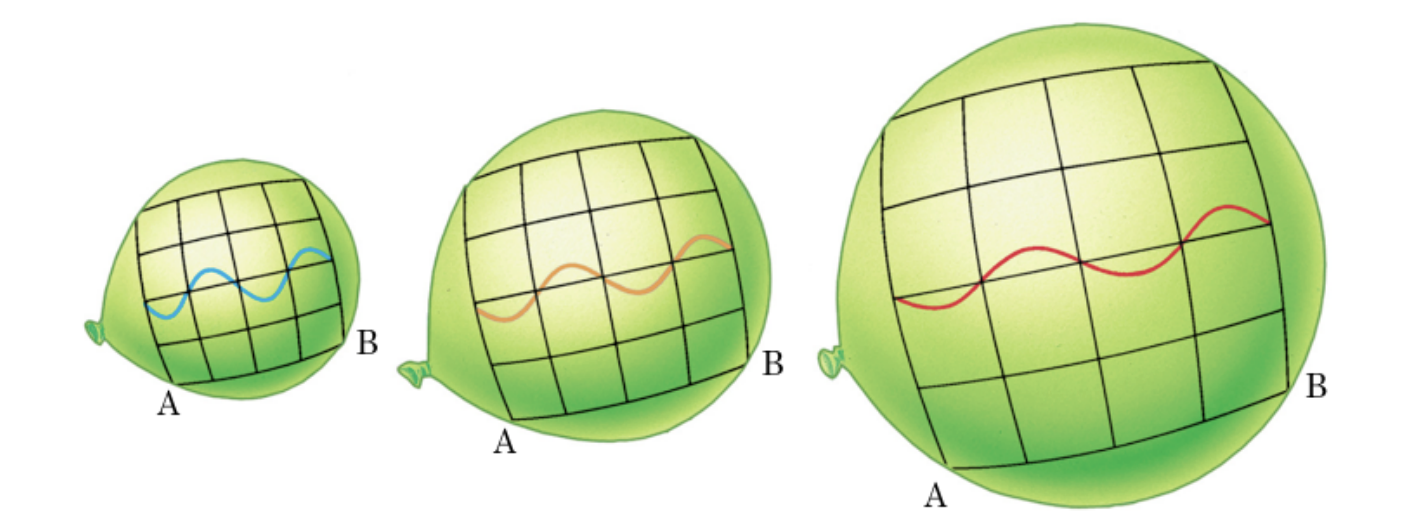
\includegraphics[width=0.65\textwidth]{images/balloon_expansion.png}
        \caption{The balloon analogy for the expansion of the universe.}
\end{figure}

\bigskip\noindent
\begin{remark}
    Although scale factor $a(t)$ can change with time, we assume that the curvature constant $k$ does not change with time, which means the geometry of the universe is fixed. \\
\end{remark}

\bigskip\noindent
\begin{foundation}
    If we consider the distance light travel from source to observer, that means $ds^2 = 0$ as light travels along null geodesics, and we can get:
    \begin{align*}
         0 &= -dt^2 + a^2(t) d\chi^2 \\
         dt &= \pm a(t) d\chi
    \end{align*}
    Note when time increase $(dt > 0)$, the light is traveling towards the observer $(d\chi < 0)$, so we need to choose the -ve sign to get the correct direction of light travel. \\

    Hence, we can get the relation between the comoving distance $\chi$ of 2 points and the time of travel $t$:
    \begin{align*}
        dt &= - a(t) d\chi \\
        \int_{\chi_0}^{\chi_{source}} d\chi  &= - \int_{t_{obs}}^{t_{emit}} \frac{dt}{a(t)} \\
        - \chi_{source} &= - \int_{t_{obs}}^{t_{emit}} \frac{dt}{a(t)} \\
        \chi_{source} &= \int_{t_{emit}}^{t_{obs}} \frac{dt}{a(t)} 
    \end{align*}
    where $\chi_{source}$ is the comoving coordinate of the source, $\chi_0$ is the comoving coordinate of the observer, and we can set $\chi_0 = 0$ for simplicity. \\
\end{foundation}

\bigskip\noindent
\begin{theory}
    To calculate the \textbf{time-independent} comoving distance $\chi$ between the source and the observer, we can use the following formula:
    \[
        \chi = \int_{t_{emit}}^{t_{obs}} \frac{dt}{a(t)} 
    \]
    which is the integral of the inverse of the scale factor over the time of travel. \\

    Note that the comoving distance $\chi$ is fixed once we defined a specific source and observer, and it does not change with time or changing scale factor, which quites counter-intuitive, but it is because the comoving distance is defined in a way that it is not affected by the expansion of the universe, and it is a measure of the distance between two points in the universe that is independent of the expansion. \\
\end{theory}

% ═════════════════════════════════════════════════════════════════════════════
%\newpage
\bigskip\noindent \bigskip\noindent \bigskip\noindent
\section{Hubble's Law}
\subsection{Redshift and Recession Velocity}
Recall the redshift $z$ can occur when the source is moving away from the observer.
\begin{foundation}
    To derive the Doppler redshift formula in special relativity, we define:
    \[
        \beta \equiv \frac{v}{c}, \qquad \gamma \equiv \frac{1}{\sqrt{1-\beta^2}}
    \]
    where $v>0$ means the source is receding from the observer. \\

    Let two successive wave crests be emitted with proper time interval $\Delta\tau_{emit}$ in the source rest frame:
    \[
        \Delta\tau_{emit} = \frac{1}{\nu_{emit}}
    \]
    In the observer frame, this emission interval is time-dilated:
    \[
        \Delta t_{emit} = \gamma\,\Delta\tau_{emit}
    \] \\
    
    \textbf{Why do we need the extra travel time?} \\
    The key insight is that between the emission of the first crest at time $t_1$ and the second crest at time $t_1 + \Delta t_{emit}$, the source is \textit{moving away} from the observer. 
    Therefore, the second crest is emitted from a point that is farther from the observer by a distance $\Delta d = v\Delta t_{emit}$.
    Since the second crest must travel this extra distance at the speed of light $c$, 
    it requires an additional time to reach the observer. \\
    
    During this interval, the source moves farther by $v\Delta t_{emit}$, so the second crest has extra travel time:
    \[
        \Delta t_{extra} = \frac{v\Delta t_{emit}}{c} = \frac{v}{c}\Delta t_{emit} = \beta\,\Delta t_{emit}
    \]
    This is the additional travel time caused by the source's recession --- the source ``runs away'' from its own light.
    Hence the observed arrival interval is:
    \[
        \Delta t_{obs} = \Delta t_{emit} + \Delta t_{extra} = \Delta t_{emit}(1+\beta)
        = \gamma\Delta\tau_{emit}(1+\beta)
    \]
    Therefore,
    \[
        \nu_{obs} = \frac{1}{\Delta t_{obs}} = \frac{1}{\gamma\Delta\tau_{emit}(1+\beta)} =\frac{\nu_{emit}}{\gamma(1+\beta)}
        = \nu_{emit}\sqrt{\frac{1-\beta}{1+\beta}}
    \] \\

    Using $\lambda = c/\nu$, we get:
    \[
        \frac{\lambda_{obs}}{\lambda_{emit}} = \frac{\nu_{emit}}{\nu_{obs}} = \sqrt{\frac{1+\beta}{1-\beta}}
    \]
    By definition of redshift,
    \[
        z \equiv \frac{\lambda_{obs}-\lambda_{emit}}{\lambda_{emit}} = \frac{\lambda_{obs}}{\lambda_{emit}} - 1
        = \sqrt{\frac{1+\beta}{1-\beta}} - 1
        = \sqrt{\frac{1+v/c}{1-v/c}} - 1
    \]
    Note $\nu$ and $v$ are 2 different things, $\nu$ is the frequency of the light wave, while $v$ is the velocity of the source. Don't mix them even they look like same!
\end{foundation}

\bigskip\noindent
\begin{theory}
    calculation on \textbf{Doppler redshift}, based on wavelength:
    \[
        z = \frac{\lambda_{obs} - \lambda_{emit}}{\lambda_{emit}} = \frac{\lambda_{obs}}{\lambda_{emit}} - 1
    \]
    and based on frequency:
    \[
        z = \frac{\nu_{emit} - \nu_{obs}}{\nu_{obs}} = \frac{\nu_{emit}}{\nu_{obs}} - 1
    \]
    and based on the peculiar velocity of the source:
    \[
        z = \sqrt{\frac{1 + v/c}{1 - v/c}} - 1
    \]
    where +ve $v$ means the source is moving away from the observer, and -ve $v$ means the source is moving towards the observer. \\
\end{theory}

% -─────────────────────────────────────────────────────────────────────────────
\bigskip\noindent \bigskip\noindent \bigskip\noindent
\subsection{Cosmological Redshift}
%\bigskip\noindent
\begin{intuition}
    However, in 1929, Edwin Hubble found that most of the galaxies are moving away from us, which does not make sense, if the doppler effect is the only reason for the redshift, then we should expect around half of the galaxies are moving towards us, and the other half are moving away from us, which is not what we observed. \\

    It suggests that there must be another reason for the redshift, and later we know that it is the expansion of the universe that causes the redshift, which dominates over the doppler effect for distant galaxies, and thats why most of the galaxies are moving away from us. \\
\end{intuition}

\bigskip\noindent
\begin{foundation}
    Start from the FLRW metric and consider radial light propagation ($d\Omega = 0$):
    \[
        ds^2 = -dt^2 + a^2(t) d\chi^2
    \]
    For photons, $ds^2 = 0$, so:
    \[
        d\chi = \frac{dt}{a(t)}
    \] \\

    Let a source at fixed comoving coordinate $\chi_s$ emit two successive crests. \\
    For the first crest (emitted at $t_{emit}$, observed at $t_{obs}$):
    \[
        \int_{t_{emit}}^{t_{obs}} \frac{dt}{a(t)} = \chi_s
    \]
    For the second crest (emitted at $t_{emit}+\Delta t_{emit}$, observed at $t_{obs}+\Delta t_{obs}$):
    \[
        \int_{t_{emit}+\Delta t_{emit}}^{t_{obs}+\Delta t_{obs}} \frac{dt}{a(t)} = \chi_s
    \]
    Because both crests travel between the same source and observer, the comoving distance is the same. Subtract the two equations:
    \[
        \int_{t_{emit}}^{t_{emit}+\Delta t_{emit}} \frac{dt}{a(t)}
        =
        \int_{t_{obs}}^{t_{obs}+\Delta t_{obs}} \frac{dt}{a(t)}
    \]
    For two \,successive crests, $\Delta t$ is very small, so $a(t)$ is nearly constant during each small interval:
    \[
        \frac{\Delta t_{emit}}{a(t_{emit})} \approx \frac{\Delta t_{obs}}{a(t_{obs})}
        \quad \Rightarrow \quad
        \frac{\Delta t_{obs}}{\Delta t_{emit}} = \frac{a(t_{obs})}{a(t_{emit})}
    \] \\

    Now convert to wavelength. For a locally measured light wave, $\lambda = c\,\Delta t$ (or $\lambda \propto \Delta t$ in $c=1$ units), therefore:
    \[
        \frac{\lambda_{obs}}{\lambda_{emit}} = \frac{\Delta t_{obs}}{\Delta t_{emit}} = \frac{a(t_{obs})}{a(t_{emit})}
    \]
    By the definition of redshift:
    \[
        z \equiv \frac{\lambda_{obs}-\lambda_{emit}}{\lambda_{emit}}
        = \frac{\lambda_{obs}}{\lambda_{emit}} - 1
        = \frac{a(t_{obs})}{a(t_{emit})} - 1
    \]
\end{foundation}


\bigskip\noindent
\begin{theory}
    Calculation on \textbf{cosmological redshift}, based on the expansion of the universe:
    \[
        z = \frac{a(t_{obs})}{a(t_{emit})} - 1 = \frac{\lambda_{obs}}{\lambda_{emit}} - 1 = \frac{\nu_{emit}}{\nu_{obs}} - 1
    \]
    and based on the recession velocity of the source:
    \[
        z = \sqrt{\frac{1 + v/c}{1 - v/c}} - 1
    \]
    where $a(t_{obs})$ is the scale factor at the time of observation, and $a(t_{emit})$ is the scale factor at the time of emission. \\

    If we treat the scale factor $a(t)$ will change with time, and let the time of observation be $t_0$, so that $a(t_0) = a_0 = 1$, then we can rewrite the cosmological redshift as:
    \[
        z = \frac{1}{a(t_{emit})} - 1
    \]
\end{theory}

\clearpage
%\bigskip\noindent
\begin{remark}
    The redshift $z$ of galaxies can be contributed by both recession motion(\textbf{cosmological redshift}) and peculiar motion(\textbf{doppler redshift}), but for distant galaxies $ z > 0.01 $, the cosmological redshift dominates over the doppler redshift.
\end{remark}
% -─────────────────────────────────────────────────────────────────────────────
\bigskip \noindent \bigskip \noindent \bigskip \noindent 
\subsection{Hubble's Law}
\begin{intuition}
    In 1823, Olber's paradox was proposed, which states that if the universe is infinite and static, then the night sky should be bright because there are infinite number of stars in the universe.  However, the night sky is dark, which means the universe cannot be infinite and static. \\

    The paradox can not be resolved until the discovery by Edwin Hubble in 1929, who found that the recession velocity of galaxies is proportional to their distance from us, which is now known as Hubble's law. The Hubble's law then become one of the core evidences for the expansion of the universe, and suggest the Big Bang theory as the most plausible model for the origin of the universe, which solves the Olber's paradox by proposing that the universe is neither infinite nor static, but it is expanding from a hot and dense initial state.
\end{intuition}

\begin{figure}[htbp]
    \centering
    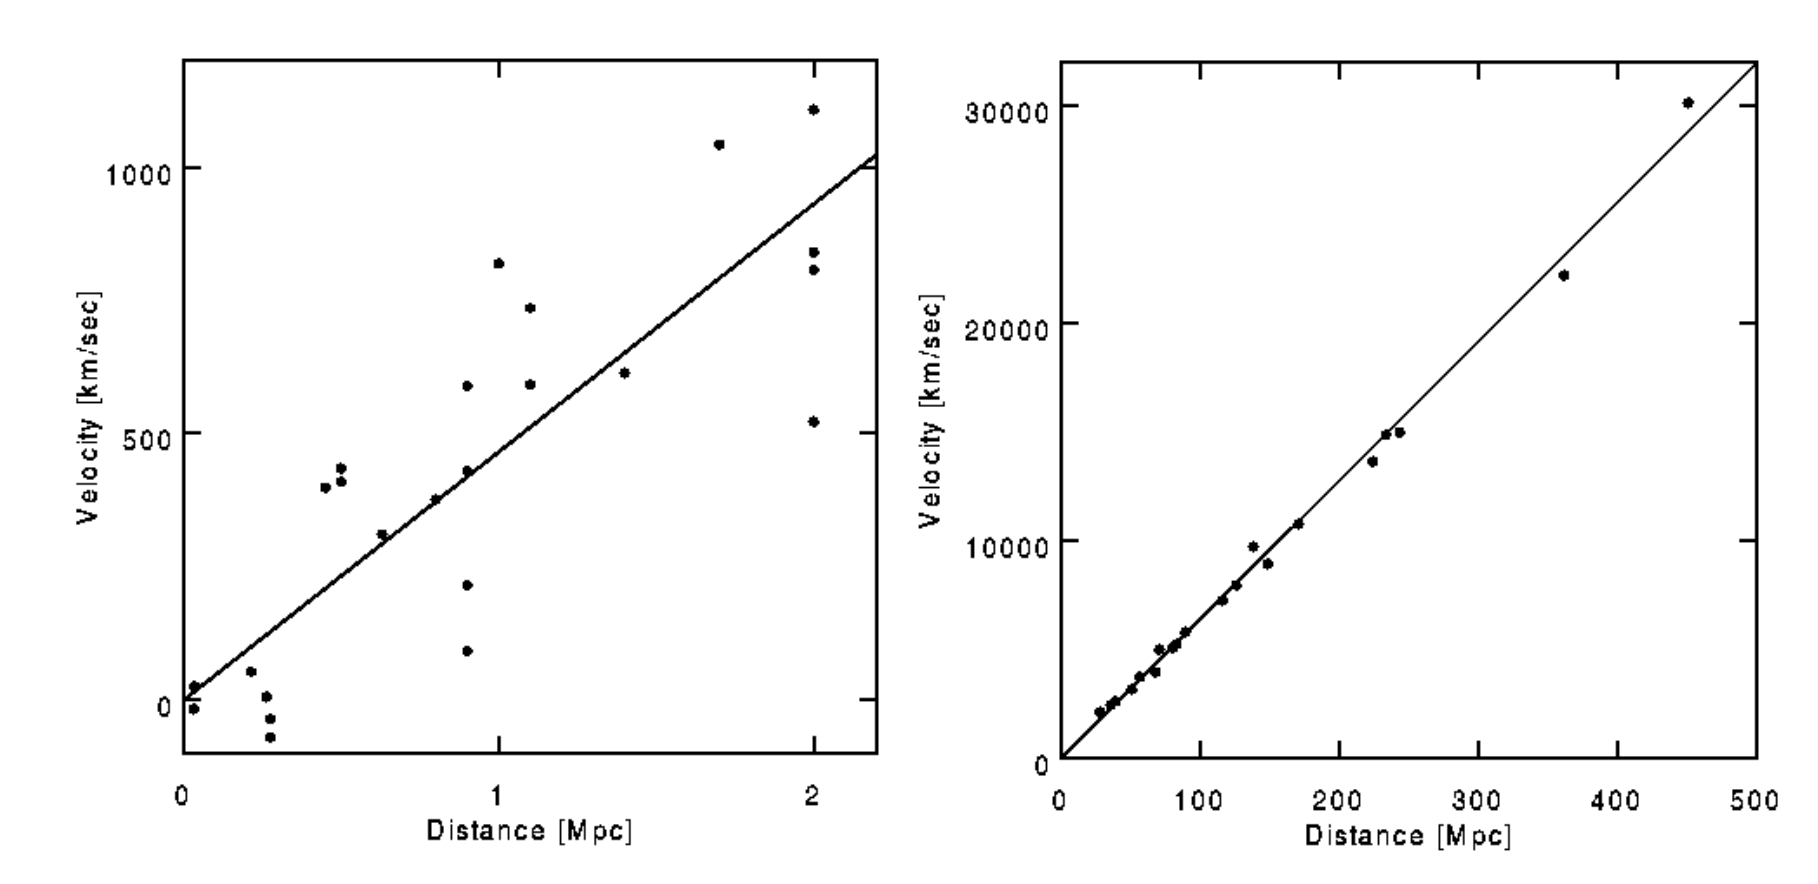
\includegraphics[width=0.75\textwidth]{images/hubble_diagram.png}
    \caption{Hubble diagram showing the relationship between the recession velocity of galaxies and their distance from us.}
    \label{fig:hubble-diagram}
\end{figure}

\bigskip\noindent
The left plot show the original data from Hubble's 1929 paper, and the right plot show the modern data from more distinct galaxies, which is more accurate and has more convincing straight line to fit.
    
\bigskip\noindent
\begin{theory}
    Hubble's Law states that the recession velocity of a galaxy is proportional to its distance from us:
    \[
        v = H D
    \]
    where $H$ is the Hubble constant, D is the proper distance to the galaxy(true distance between 2 points), and can be changed with time unlike the co-moving distance(the number of marks).
\end{theory}

\bigskip\noindent
\begin{theory}
    Let $D_{proper}$ be the proper distance to a galaxy, and $\chi$ be the co-moving distance coordinate to the galaxy, then we have:
    \[
        D_{proper}(t) = a(t) \cdot \chi
    \] 
    Note $\chi$ is independent to time.\\

    The recession velocity $v$ can also be defined as:
    \[
        v \equiv \frac{dD_{proper}}{dt} = \dot{a}(t) \cdot \chi
    \]
    And sub the Hubble's law into the above equation, we can get:
    \begin{align*}
        v &= H D_{proper} \\     
        \dot{a}(t) \cdot \chi &= H a(t) \cdot \chi \\
        \dot{a}(t) &= H a(t)
    \end{align*} 

    And we know that the Hubble parameter is equal to:
    \[
        H(t) = \frac{\dot{a}(t)}{a(t)} = - \frac{\dot{z}(t)}{1 + z(t)}
    \]
\end{theory}

\bigskip\noindent
\begin{remark}
   For $t > 0$ (after Big Bang), $a(t) > 0$, except at the initial singularity$(t = 0, a(0) = 0)$; \\
   
   while the observation shows that $H_0 > 0$, which indicates $\dot{a}(t_0) > 0$, which means the universe is expanding at the current time $t_0$.
\end{remark}

\clearpage
%\bigskip\noindent
Now we can finding the relationship between the redshift $z$ and the distance $D$ of a galaxy, by using the Hubble's law and the definition of cosmological redshift:
\begin{theory}
    we have cosmological redshift:
    \[
        z = \frac{1}{a(t_{emit})} - 1
    \]
\end{theory}

\bigskip\noindent
\begin{importantnote}
    Hubble's constant $H_0$ is not actually a constant, but it can change with time. \\

    The value of $H(t_0) = H_0$ is the current value of the Hubble parameter, which is measured to be around $67.66 \pm 0.42 \, \mathrm{km/s/Mpc}$ by the Planck Mission in 2018.
\end{importantnote}
    
\bigskip\noindent
\begin{extra}
    The Hubble's law get renamed to Hubble-Lemaître law in 2018 by the International Astronomical Union (IAU) to recognize the contribution of Georges Lemaître, who first derived the linear relationship between the recession velocity and distance of galaxies in 1927, two years before Hubble's observational discovery in 1929. However, the name change is still controversial, and many people still refer to it as Hubble's law. 
\end{extra}

\bigskip\noindent
\begin{extra}
    The Hubble's constant can not be measured directly, but it can be inferred indirectly through observations of the universe, and there are two main methods: the distance ladder method and the cosmic microwave background (CMB) method. \\

    The distance ladder method uses standard candles like Cepheid variables and Type Ia supernovae to measure the distance to galaxies, it focus on "late universe", which means the universe at low redshift$z < 0.1$, and get the value of the Hubble constant to be around $73.04 \pm 1.04 \, \mathrm{km/s/Mpc}$ by the SH0ES team in 2021. \\

    The CMB method uses the anisotropies in the cosmic microwave background radiation to infer the value of the Hubble constant, it focus on "early universe", which means the universe at high redshift $z \sim 1100$, and get the value of the Hubble constant to be around $67.66 \pm 0.42 \, \mathrm{km/s/Mpc}$ by the Planck Mission in 2018. \\

    The difference results of $H_0$ obtained by two methods is known as the Hubble tension, which is one of the biggest unsolved problems in cosmology.
\end{extra}
\clearpage